\chapter{Digital-Analog Wandler / Analog-Digital Wandler}
\textbf{Beispiel Musikspeicherung} \\
Schwallwellen $\rightarrow$ Mikrophon (Spannung - analoges Signal) $\rightarrow$ MP3-Datei (Bit 0/1 - digitales Signal) $\rightarrow$ DA-Wandler $\rightarrow$ Lautsprecher (analoges Signal)

\begin{figure}[H]
	\centering
	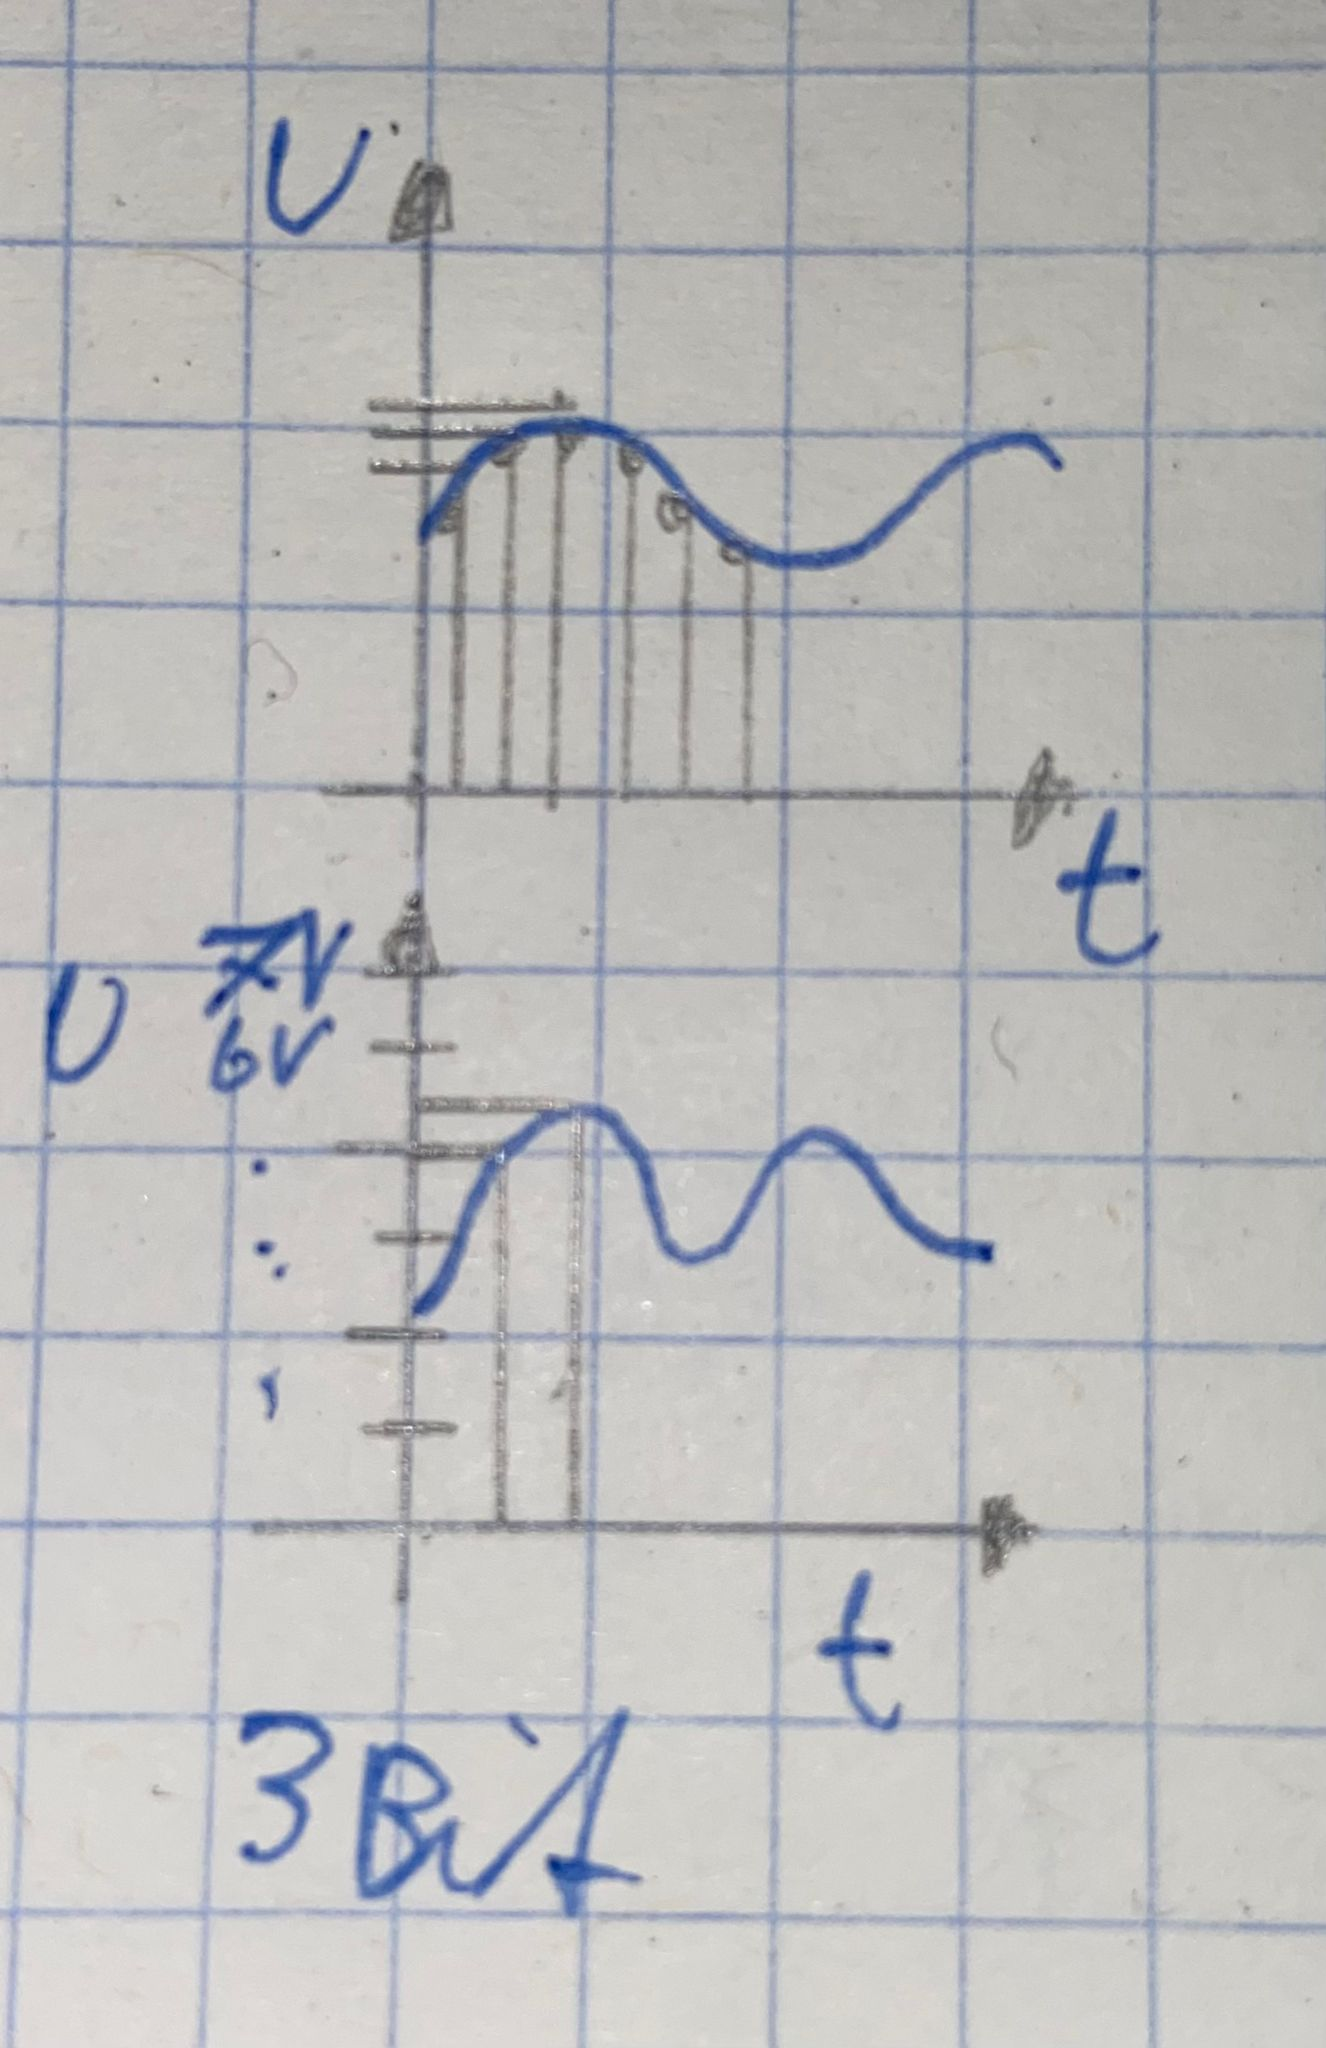
\includegraphics[width=0.2\linewidth]{figures/daad1.jpeg}
	\caption{DA/AD-Wandler}
\end{figure}

\begin{itemize}
	\item Pegel messen
	\item Binärzahl speichern
	\item je höher die Abtastrate (Samplerate) desto besser
	\item je mehr Bits zum Speichern verwendet werden, desto genauer
\end{itemize}
Typische Abtastrate: ca. 44 kHz

\section{Digital-Analog Wandler}
Aufgabe: muss aus einer Binärzahl eine Spannung erzeugen

Bsp: 2 Bit Spannung 0-5 Volt \\
00 $\rightarrow$ 0V \\
01 \\
10 \\
11 $\rightarrow$ 5V \\ \\
$\Rightarrow$ $\dfrac{5}{3}$ = $\Delta$U ... Schrittgröße
\begin{center}
	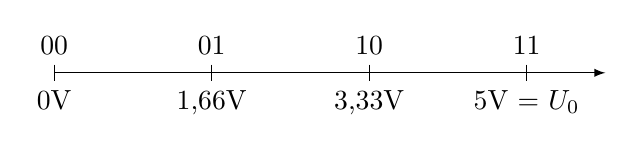
\begin{tikzpicture}
		\draw[-latex] (0,0) -- (7,0); %edit here for the axis
		\foreach \x in  {0,2,4,6} % edit here for the vertical lines
		\draw[shift={(\x,0)},color=black] (0pt,3pt) -- (0pt,-3pt);
		
		\draw (0,0) node[above=3pt]{00};
		\draw (2,0) node[above=3pt]{01};
		\draw (4,0) node[above=3pt]{10};
		\draw (6,0) node[above=3pt]{11};
		
		\draw (0,0) node[below=3pt]{0V};
		\draw (2,0) node[below=3pt]{1,66V};
		\draw (4,0) node[below=3pt]{3,33V};
		\draw (6,0) node[below=3pt]{5V = $\text{U}_0$};
	\end{tikzpicture}
\end{center}

Je mehr Bit, desto besser kann man den Spannungsbereich abdecken \\

\textbf{Allgemein:} Schrittgröße: $\Delta$U = $\dfrac{\text{U}_0}{2^{\text{n}}-1}$ \\
\textbf{maximaler Fehler:} $\text{F}_{\text{max}}$ = $\dfrac{\Delta \text{U}}{2}$

\textbf{Aufbau eines DA-Wandlers} \\
z.B. 3 Bit, $\text{U}_0$ = 5 Volt \\
zur Vereinfachung: $\Delta$U = $\dfrac{\text{U}_0}{2^{\text{n}}}$ statt $\Delta$U = $\dfrac{\text{U}_0}{2^{\text{n}}-1}$ \\

$\Delta$U = $\dfrac{5}{2^{3}}$ = $\dfrac{5}{8}$V = 0,625V

\begin{tabular}{|c|c|r|}
	\hline
	\textbf{Deziaml} & \textbf{Eingang} & \textbf{Ausgang} \\
	\hline
	0 & 000 & 0V \\ 
	\hline
	1 & 001 & 0,625V \\ 
	\hline
	2 & 010 & 1,25V \\ 
	\hline
	3 & 011 & 1,875V \\ 
	\hline
	4 & 100 & 2,5V \\ 
	\hline
	5 & 101 & 3,125V \\
	\hline
	6 & 110 & 3,75V \\
	\hline
	7 & 111 & 4,375V \\
	\hline
\end{tabular}

110 = 2,5 + 1,25 = 3,75V \\

\textbf{Schaltung eines DA-Wandlers} \\
\begin{figure}[H]
	\centering
	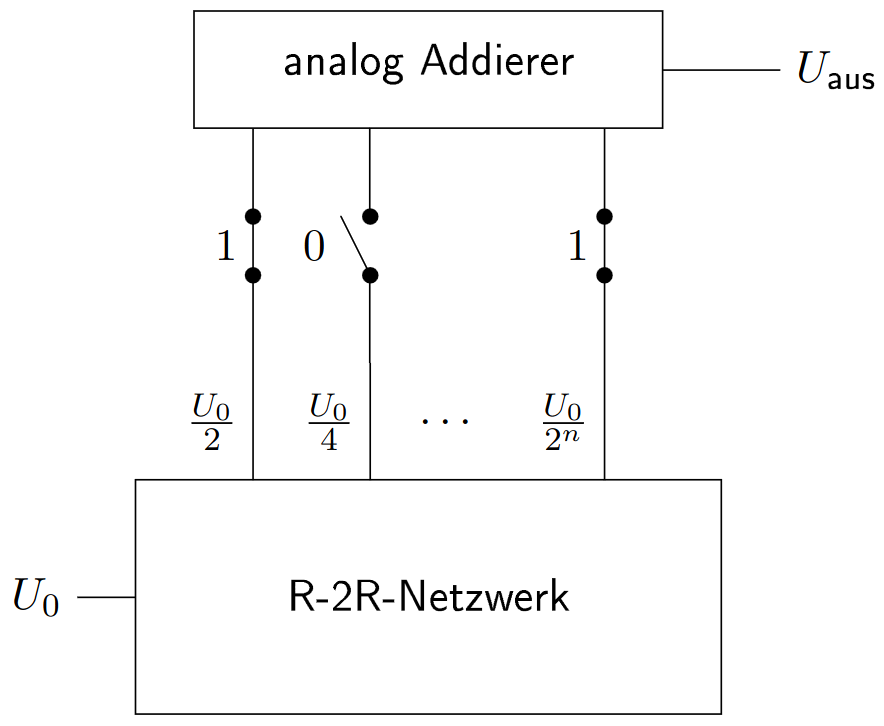
\includegraphics[width=0.8\linewidth]{figures/da_wandler.png}
	\caption{DA-Wandler}
\end{figure}

Schaltung wo die Spannung immer halbiert wird. \\
Idee: gleich große Widerstände in einer Reihenschaltung

\begin{figure}[H]
	\centering
	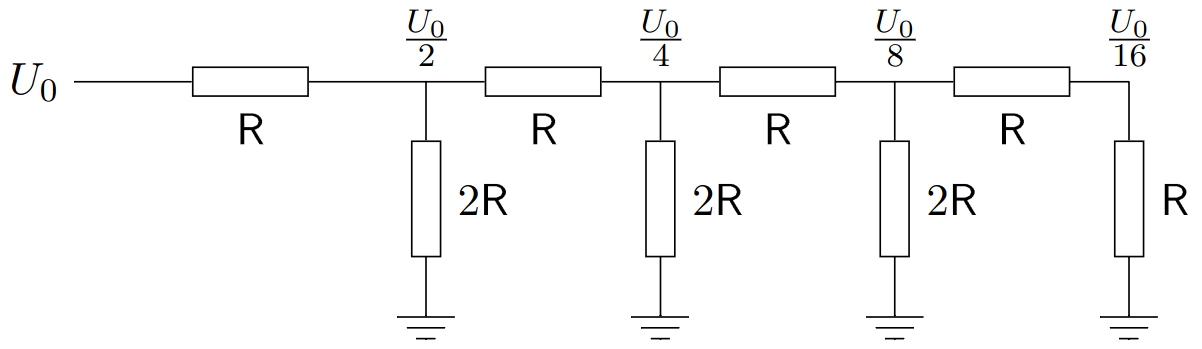
\includegraphics[width=0.8\linewidth]{figures/r2r.png}
	\caption{R-2R-Netzwerk}
\end{figure}

Beispiel: DA-Wandler 8 Bit, $\text{U}_0$ = 10V \\
\begin{enumerate}
	\item Wie groß ist eine Schrittgröße? ($\Delta$U) \\
	$\Delta$U = $\dfrac{10}{2^{8}}$ = 0,039625V
	\item Wie groß ist der maximale Fehler? \\
	$\text{F}_{\text{max}}$ = $\dfrac{0,039625}{2}$ = 0,01953125V (außer ganz oben bei 10V, $\Delta$U)
	\item Welche Spannung erzeugt die Eingabe von 10011101? \\
	$(\text{10011101})_2$ = $(\text{157})_{10}$ \\
	$\text{U}_{\text{aus}}$ = 157$\cdot$$\Delta$U = 6,221125V
	\item Welche Binärzahl wird für 8V verwendet und wie groß ist der Fehler? \\
	$\dfrac{8}{\Delta\text{U}}$ = $(\text{204,8})_{10}$ $\approx$ $(\text{205})_{10}$ = $(\text{11001101})_2$ \\ \\
	8V = x$\cdot$$\Delta$U $\Rightarrow$ 205$\cdot$$\Delta$U = 8,123125 \\
	Fehler = 8,123125 - 8 = 0,123125V
	\item Wei viele Bits benötigt man damit der Fehler kleiner als 2mVist? Wie groß ist der Fehler? \\
	n = ?, $\text{U}_0$ = 10V, $\text{F}_{\text{max}}$ $\le$ 2mV \\
	$\text{F}_{\text{max}}$ $\le$ 2mV \\
	$\dfrac{\Delta\text{U}}{2}$ = $\dfrac{\text{U}_0}{\dfrac{2^\text{n}}{2}}$ $\le$ 2mV \quad$\vert$ $\cdot$2 \\
	$\dfrac{\text{U}_0}{2^\text{n}}$ $\le$ 0,004 V \quad$\vert$ $\cdot$$2^\text{n}$ \quad$\vert$/0,004 \\
	$\dfrac{10}{0,004}$ = $2^\text{n}$ \quad ln \\
	ln(2500) = n$\cdot$ln(2) \quad$\vert$/ln(2) \\
	$\dfrac{ln(2500)}{ln(2)}$ = n \\
	11,2577 = n \\
	n $\approx$ 12 \\
	
	$\Delta$U = $\dfrac{\text{U}_0}{2^\text{n}}$ = $\dfrac{10}{2^{12}}$ = 2,44 mV \\
	
	$\text{F}_{\text{max}}$ = $\dfrac{ \dfrac{10}{2^{12}} }{2}$ = 1,22 mV

\end{enumerate}

\section{Analog-Digital Wandler}
Der Analog-Digital Wandler muss beliebige Werte (analoges Signal) in eine Binärzahl übersetzen.

Bsp:
$\text{U}_0$ = 5V, 2 Bit ($2^{2}$ = 4 Zahlen: 00, 01, 10, 11) \\
$\Delta$U = $\dfrac{5}{4}$ = 1,25 V

\begin{center}
	\begin{tikzpicture}[scale=2,% for curly brackets
		> = Straight Barb,
		BC/.style args = {#1/#2}{
			decorate,
			decoration={calligraphic brace, amplitude=6pt,
				pre =moveto, pre  length=1pt,
				post=moveto, post length=1pt,
				raise=#1,
				#2,
			},
			ultra thick},
		]
		\draw[-latex] (0,0) -- (5.5,0); %edit here for the axis
		\foreach \x in {0,1.25,2.5,3.75,5} % edit here for the vertical lines
		\draw[shift={(\x,0)},color=black] (0pt,3pt) -- (0pt,-3pt);
		
		\draw[BC=4pt/] (0,0) -- node[above=7pt] {00} (1.25,0); 
		\draw[BC=4pt/] (1.25,0) -- node[above=7pt] {01} (2.5,0); 
		\draw[BC=4pt/] (2.5,0) -- node[above=7pt] {10} (3.75,0); 
		\draw[BC=4pt/] (3.75,0) -- node[above=7pt] {11} (5,0); 
		
		\draw (0,0) node[below=3pt]{0};
		\draw (1.25,0) node[below=3pt]{1,25};
		\draw (2.5,0) node[below=3pt]{2,5};
		\draw (3.75,0) node[below=3pt]{3,75};
		\draw (5,0) node[below=3pt]{5};
	\end{tikzpicture}
\end{center}

Erste Schritt = $\dfrac{\Delta\text{U}}{2}$

\begin{center}
	\begin{tikzpicture}[scale=2,% for curly brackets
		> = Straight Barb,
		BC/.style args = {#1/#2}{
			decorate,
			decoration={calligraphic brace, amplitude=6pt,
				pre =moveto, pre  length=1pt,
				post=moveto, post length=1pt,
				raise=#1,
				#2,
			},
			ultra thick},
		]
		\draw[-latex] (0,0) -- (5.5,0); %edit here for the axis
		\foreach \x in {0,0.625,1.875,3.125,5} % edit here for the vertical lines
		\draw[shift={(\x,0)},color=black] (0pt,3pt) -- (0pt,-3pt);
		
		\draw[BC=4pt/] (0,0) -- node[above=7pt] {00} (0.625,0); 
		\draw[BC=4pt/] (0.625,0) -- node[above=7pt] {01} (1.875,0); 
		\draw[BC=4pt/] (1.875,0) -- node[above=7pt] {10} (3.125,0); 
		\draw[BC=4pt/] (3.125,0) -- node[above=7pt] {11} (5,0); 
		
		\draw (0,0) node[below=3pt]{0};
		\draw (0.625,0) node[below=3pt]{0,625};
		\draw (1.875,0) node[below=3pt]{1,875};
		\draw (3.125,0) node[below=3pt]{3,125};
		\draw (5,0) node[below=3pt]{5};
	\end{tikzpicture}
\end{center}

\begin{center}
\begin{tikzpicture}
	\def\x{1.25}
	\begin{axis}[
		axis lines = left,
		xlabel = U,
  		xtick={0,\x,\x*2,\x*3,\x*4},
		ylabel = D,
  		ytick={0,1,2,3},
  		yticklabels={00,01,10,11},
  		ymax=3.5,
  		xmax=5.5
		]

		\addplot [
		domain=0:5, 
		samples=10, 
		color=blue,
		]
		{0.6*x};

		\addplot[color=gray,mark=none] coordinates { (0,0) (\x,0)};
		
  		\addplot[color=gray,mark=none] coordinates { (\x,0) (\x,1)};
  		\addplot[color=gray,mark=none] coordinates { (\x,1) (\x*2,1)};
		
		\addplot[color=gray,mark=none] coordinates { (\x*2,1) (\x*2,2)};
		\addplot[color=gray,mark=none] coordinates { (\x*2,2) (\x*3,2)};

		\addplot[color=gray,mark=none] coordinates { (\x*3,2) (\x*3,3)};
		\addplot[color=gray,mark=none] coordinates { (\x*3,3) (\x*4,3)};
\end{axis}
\end{tikzpicture}
\end{center}
Fehler: fast $\Delta$U (?)

\begin{center}
\begin{tikzpicture}
	\def\x{0.625}
	\begin{axis}[
		axis lines = left,
		xlabel = U,
    	xticklabel style={/pgf/number format/.cd,fixed,precision=3},
		xtick={0, \x, \x*3, \x*5, \x*8},
		ylabel = D,
		ytick={0,1,2,3},
		yticklabels={00,01,10,11},
		ymax=3.5,
		xmax=5.5
		]
		
		\addplot [
		domain=0:5, 
		samples=10, 
		color=blue,
		]
		{0.8*x};
		
		\addplot[color=gray,mark=none] coordinates { (0,0) (\x,0)};
		
		\addplot[color=gray,mark=none] coordinates { (\x,0) (\x,1)};
		\addplot[color=gray,mark=none] coordinates { (\x,1) (\x*3,1)};
		
		\addplot[color=gray,mark=none] coordinates { (\x*3,1) (\x*3,2)};
		\addplot[color=gray,mark=none] coordinates { (\x*3,2) (\x*5,2)};
		
		\addplot[color=gray,mark=none] coordinates { (\x*5,2) (\x*5,3)};
		\addplot[color=gray,mark=none] coordinates { (\x*5,3) (\x*8,3)};
	\end{axis}
\end{tikzpicture}
\end{center}
Fehler: $\dfrac{\delta\text{U}}{2}$, außer am Ende

\subsection{Verfahren und Schaltungen}
\begin{itemize}
	\item Parallelverfahren
	\item Wägeverfahren
	\item Zählerverfahren
\end{itemize}
alle Schaltungen (10 V $\rightarrow$ 3 Bit) \\
Alle benötigen zumindest einen Komparator

\begin{circuitikz}
	\draw (0,0) node[op amp, yscale=-1](comp){}
		(comp.-) -- ++(-0.5,0) node[above]{$\text{U}_2$}
		(comp.+) -- ++(-0.5,0) node[above]{$\text{U}_1$}
		(comp.out) -- ++(0.5,0) node[above]{$\text{U}_{\text{aus}}$};
\end{circuitikz}

$\text{U}_{\text{aus}}$ = 
\begin{math}
	\left\{
	\begin{array}{l}
		\text{HIGH (1)} \quad \text{U}_\text{1} \ge \text{U}_\text{2} \\
		\text{LOW (0)} \quad \text{U}_\text{1} \le \text{U}_\text{2}
	\end{array}
	\right.
\end{math}

